\chapter{Mezclas de distribuciones gausianas}

En este cap\'itulo primero se hablar\'a en t\'erminos generales sobre qu\'e es una distribuci\'on tipo mezcla. Despu\'es se hablar\'a de un caso particular de las distribuciones tipo mezcla continua, es decir, de las distribuciones tipo mezcla normal (McNeil et al, 2015). Para despu\'es caracterizar a la distribuci\'on hiperb\'olica generalizada a partir de una distribuci\'on tipo mezcla. Por \'ultimo, se aprovechar\'an algunas propiedades de las distribuciones tipo mezcla normal, para obtener algunas caracter\'isticas de inter\'es de la distribuci\'on hiperb\'olica generalizada.

\section{Distribuciones tipo mezcla }
Este tipo de distribución consiste en ponderarar un conjunto numerable de vectores aleatorios $X_{i}$  discretos con el mismo soporte y la misma dimensión con un conjunto de pesos $w_{i}$, positivos y menores a uno, $w_{i}$, donde $i$ proviene de un conjunto $I$ de índices numerable, y a su vez $\sum_{i\in I}w_{i}=1$. El índice $i$ puede ser generado por una distribución de probabilidad discreta tal que $P(i)=w_{i}$; por ello a los pesos también se les conoce como probabilidades. Entonces la función de densidad es de la siguiente forma:\\

\begin{equation*}
f_{x}(x)= \sum_{i\in I}w_{i}f_{X_{i}}(x)
\end{equation*}
Donde  $0<w_{i}<1$, $\sum_{i\in I}w_{i}=1,$ y $  f_{X_{i}}(x)$ es un vector aleatorio discreto de dimensión p para todo $i$ en $I$.\\

Es común encontrar este tipo de distribuciones en un conjunto de datos que provienen de dos o más distribuciones diferentes, lo cual podría resultar en una distribución multimodal. Si el conjunto de vectores aleatorios provienen de la misma distribución, entonces se dice que es una mezcla de familias paramétricas, mientras que si el vector aleatorio tiene una distribución continua se le conoce como densidad tipo mezcla continua.\\
Una densidad tipo mezcla continua resulta de considerar que los pesos $w$ están dados por una densidad continua $f_{w}(w)$ con soporte en $R_{+}$; a $w$ se le conoce como variable de mezcla. Ahora, el vector aleatorio $X$ está parametrizado por $(\theta,w)$, por lo que la familia de vectores aleatorios queda determinada por la familia no numerable  $ X$ dado $w$, con $w$ distribuido $f_{w}(w) $. Entonces, la densidad de $X$ esté dada por:\\
\begin{equation*}
f_{x}(x)=\int_{0}^{\infty}f(x|w)f_{w}(w)dw 
\end{equation*}


Si $w$ es una variable aleatoria con distribución paramétrica, es común que la distribución de $X$ dependa de los parámetros de $u$, y además ciertas características como la dispersión o la cola de la distribución de $X$ también dependan de las características de la variable de mezcla $w$.\\

\section{Mezcla gaussiana en media}
Se dice que un vector aleatorio $X$, de dimensión $p$, es una mezcla en media si, dado $u$, $X$ tiene una distribución gaussiana con vector de  medias $u\mu$, y matriz de varianza-covarianza $\Sigma$. La variable aleatoria $u$ está definida en $R_{+}$. Entonces la probabilidad de que $X$ pertenezca a algún subconjunto $S_{p}\subset  R^{p}$ es:

\begin{equation*}
P((X_{1},...,X_{p})\in S_{p})=\underset{0}{\overset{\infty }{\int }}N_{p}(X \in S_{p} |u\mu,\Sigma)f_{u}(u)du, 
\end{equation*}
donde  $\mu \in R^{p}$, $\Sigma \in M_{p\times p}$ y $u$ es la variable de mezcla.\\
Si nos enfocamos en la distribución marginal de $X$ dado $u$ podemos notar que el valor de $u$ influye en donde está centrada la distribución, pues ahora el vector de medias pertenece al segmento dirigido $L(\mu)=( u\mu | u\in R_{+}, \mu\in R^{p})$. Entonces, si consideramos que $u$ ha tomado el valor de $u_{i}$, y una muestra aleatoria de $X$ dado $u_{i}$, tendremos una muestra centrada sobre el segmento dirigido $L(\mu)$ en el punto $u_{i}\mu$, por lo que para valores de $u$ cercanos a uno, la muestra permanece centrada al rededor de $\mu$, mientras que para valores grandes de $u$, la muestra se aleja en dirección del vector de medias $\mu$. \\


En la gráfica (\ref{fig:RplotG}) se ilustra la simulación de una distribución tipo mezcla gaussiana con vector de medias $\mu=(9,11)$, matriz de varianza-covarianza $\Sigma$, con entradas $\sigma_{1}=\sigma_{2}=5$, y $\sigma_{1,2}=\sigma_{2,1}=0.1$
%$\left(
%\begin{array}{lcr}
%5 & .1 \\ .1 & 5
%\end{array}\right) $
, y con variable de mezcla distribuida exponencialmente, para tres diferentes valores de $u$. Obsérvese que para cada valor que tomó la variable de mezcla $u$, las realizaciones del vector aleatorio $X$ dado $u$ se concentrán al rededor 
de algún punto del vector de medias $u\mu$.\\   

\begin{figure}[h]
	\centering
	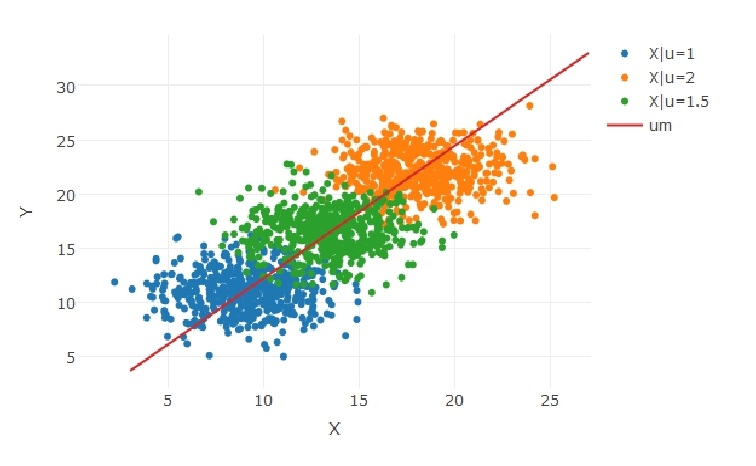
\includegraphics[width=1.15\linewidth]{Figuras/RplotG}
	\caption{Mezcla en media}
	\label{fig:RplotG}
\end{figure}

%En la gráfica (\ref{fig:mm}) se observa como tanto la función de densidad, como los contornos del vector aleatorio $X$ dado $u$, se ven afectados por la variable de mezcla $u$, para tres diferentes valores de $u$.\\

\begin{figure}[h]
	\centering
	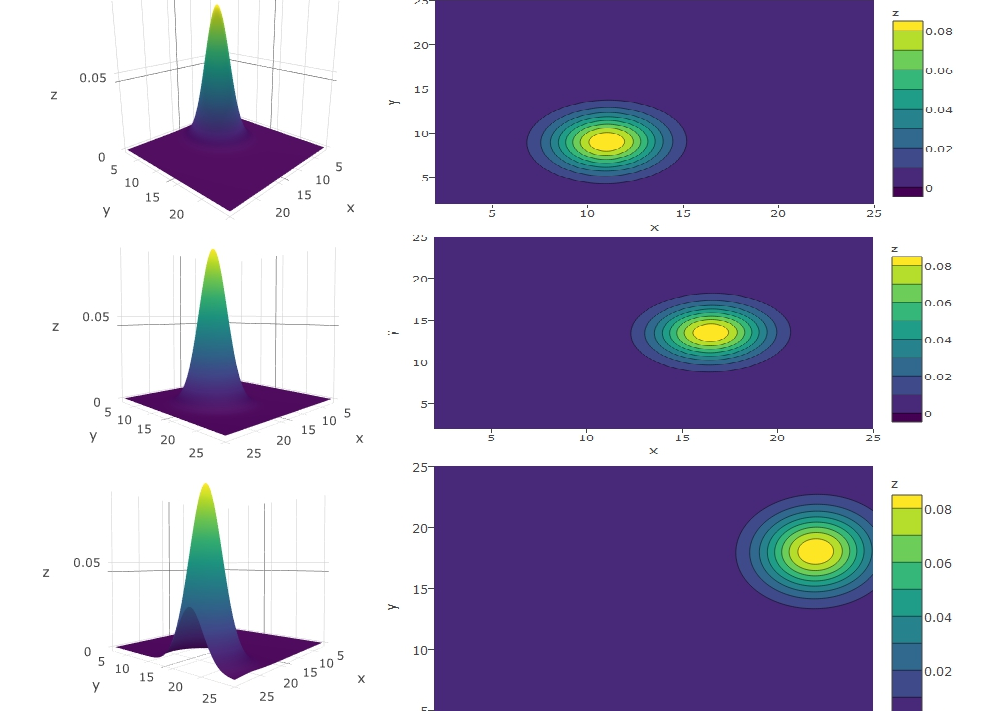
\includegraphics[width=1.15\linewidth]{Figuras/mm}
	\caption{Contornos de una distribución tipo mezcla normal en media.}
	\label{fig:mm}
\end{figure}

\pagebreak
En la gráfica (\ref{fig:mm}) se observa como tanto la función de densidad, como los contornos del vector aleatorio $X$ dado $u$, se ven afectados por la variable de mezcla $u$, para tres diferentes valores de $u$.\\

Ahora veamos analíticamente cómo influyen algunas de las caractarísticas numéricas de la variable de mezcla $u$ en la dispersión del vector aleatorio $X$, por lo que:
%%PONER ESTO EN UN ARRAY
\begin{eqnarray}
E[X]& =&\int_{0}^{\infty} \left( \int_{D_{X}}XN_{p}(X|u\mu,\Sigma)f_{u}(u)du\right)  dx \nonumber\\
&=&\int_{0}^{\infty}f_{u}(u)\left(\int_{D_{X}}XN_{p}(X|u\mu,\Sigma)f_{u}(u)dx\right)du\nonumber\\
&=&\int_{0}^{\infty}f_{u}(u)E[X|u]du\nonumber\\
&=&\int_{0}^{\infty}f_{u}(u)u\mu du\nonumber\\
&=&\mu\int_{0}^{\infty}uf_{u}(u)du\nonumber\\
&=&\mu E[u]\nonumber\\
\end{eqnarray}

%\begin{equation*}
%E[X]=\int_{0}^{\infty} \left( \int_{D_{X}}XN_{p}(X|u\mu,\Sigma)f_{u}(u)du\right)  dx
%\end{equation*}
%\begin{equation*}
%\int_{0}^{\infty}f_{u}(u)\left(\int_{D_{X}}XN_{p}(X|u\mu,\Sigma)f_{u}(u)dx\right)du=\int_{0}^{\infty}f_{u}(u)E[X|u]du
%\end{equation*}
%\begin{equation*}
%\int_{0}^{\infty}f_{u}(u)u\mu du=\mu\int_{0}^{\infty}uf_{u}(u)du=\mu E[u]
%\end{equation*}


Mientras que por el anexo $4$ se tiene que: 
\begin{eqnarray}
Cov(X)&=&E[Cov(X|u)]+Cov[E[X|u]]
\nonumber\\
&=&E[\Sigma]+Cov[u\mu]\nonumber\\
&=&\Sigma + var(u)\mu \mu',\nonumber\\
\end{eqnarray}
siempre y cuando el segundo momento de $X$ y $u$ existan. \\

Así, la variable de mezcla $u$ influye en la localización y dispersión del vector aleatorio $X$; intuitivamente podemos considerar al producto de $u$ con el vector de medias $\mu$ como un sesgo adicional que influye en la realización del vector aleatorio $X$. Este tipo de mezcla nos permite modelar conjuntos de datos que sigan alguna tendencia con disperción constante, como se ilustra en la gráfica (\ref{fig:RplotG}). Por otra parte , una de las mayores dificultades es que, salvo en algunas excepciones, no siempre existe una forma cerrada para la densidad del vector aleatorio $X$, por lo que tendría que ser aproximada mediante algún método númerico.\\

Mediante un proceso de simulación se generaron realizaciones del vector aleatorio $X$ a través de distribuciones tipo mezcla normal, lo cual se ilustra en la gráfica (\ref{fig:abcd}). La gráfica a) proviene de una variable de mezcla Exponencial con parámetro $\lambda=1.5$, la b) proviene de una variable de mezcla Gamma con parámetros $\alpha=20$, $\beta=5$, la c) provine de una variable de mezcla Pareto con parámetros $\theta=5$, $\alpha=2$, y la d) proviene de una variable de mezcla Ji-cuadrada con 20 grados de libertad (el vector aleatorio $X$ dado $u$ se distribuye de la misma manera que en la gráfica (\ref{fig:RplotG})).

\begin{figure}[h]
	\centering
	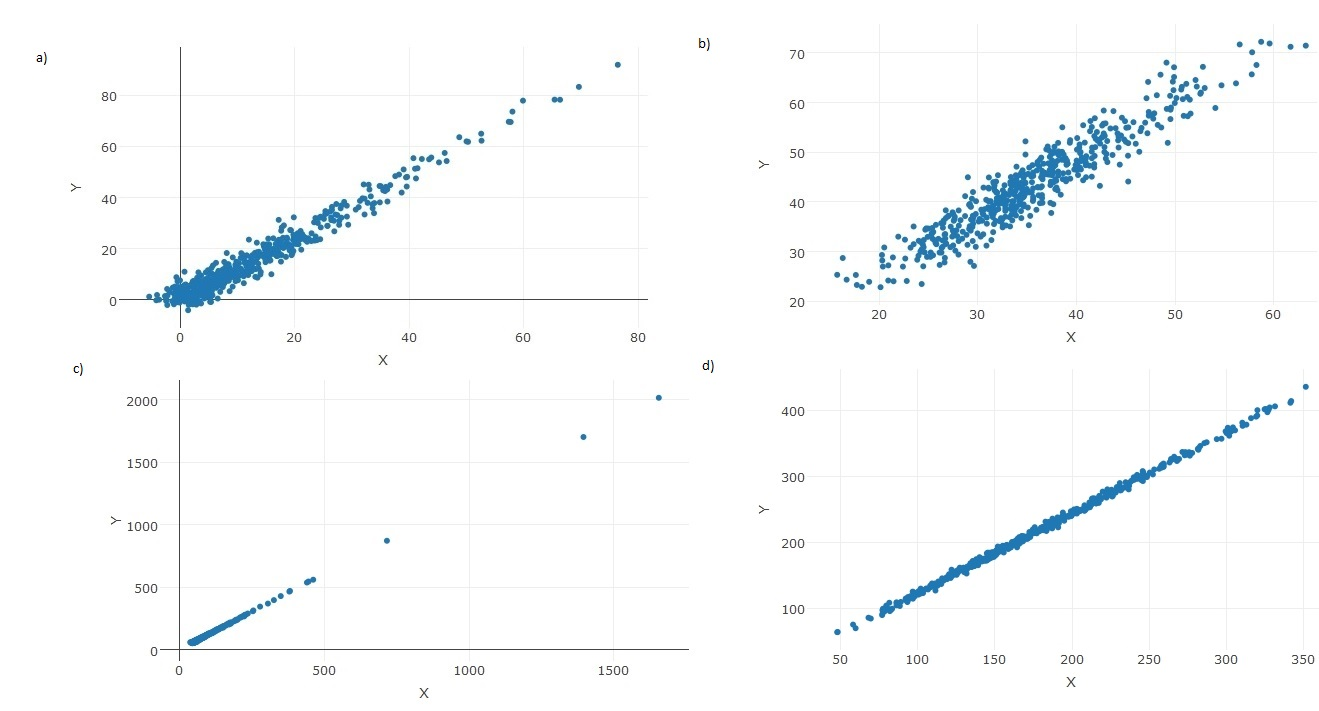
\includegraphics[width=1\linewidth]{Figuras/expo}
	\caption{Simulación del vector aleatorio X a través de distribuciones tipo mezcla normal con diferente variable de mezcla.}
	\label{fig:abcd}
\end{figure}
Como se describió en la gráfica (\ref{fig:RplotG}), las simulaciones del vector aleatorio $X$ parecen seguir una tendencia, y además es importante notar que la dispersión alrededor del vector de tendencia de la gráfica (b) es mayor a la de la gráfica (b). También es importante notar que en la gráfica (c) hay valores aparentemente grandes, mientras que en la gráfica (d) casi todos los valores parecen concentrarse en algún intervalo de la posible recta de tendencia.
Por lo que, intuitivamente la cola de la distribución de $u$ influye en la distribución de $X$. La gráfica (d) proviene de considerar una variable de mezcla distribuida Pareto, la cual tiene cola pesada, y como consecuencia podemos observar gran dispersión sobre el vector de tendencia. Mientras que la gráfica (d) proviene de considerar una variable de mezcla $u$ distribuida Xi cuadrado, que es de cola ligera, y como consecuencia las simulaciones del vector $X$ no están tan dispersas sobre el vector de tendencia (lo mismo podemos decir de la gráfica (a) y (b)).


\section{Mezcla gaussiana en varianza}
Ahora consideremos un modelo similar al anterior, pero con la diferencia que la variable de mezcla u solamente afecta a la matriz de varianza-covarianza $\Sigma$. Luego, la distribución del vector aleatorio $X$ de dimensión $p$ viene dado por:
\begin{equation}
P\left( (X_{1},...,X_{p})\in S_{p} \right )=\underset{0}{\overset{\infty }{\int }}N_{p}(X\in S_{p}|\mu,u\Sigma)f_{u}(u)du 
\end{equation}
En la distribución condicional de $X$ dado $u$, podemos notar que $u$ influye en la disperción de $X$, por lo que entre mayor sea el valor que tome $u$, mayor será la disperción al rededor del vector de medias $\mu$. Como ejemlo, en la gráfica (\ref{fig:mez}) se presenta la simulación de una variable tipo mezcla normal en varianza, con vector de medias $\mu=(9,11)$, matriz de varianza-covarianza $\sigma_{1}=\sigma_{2}=5$, y $\sigma_{1,2}=\sigma_{2,1}=0.1$
%$\Sigma = $
%$\left(
%\begin{array}{lcr}
%5 & .1 \\ .1 & 5
%\end{array}\right) 
%$
, y variable de mezcla $u$ distribuida Exponencial, con parámetro $\lambda=1$.\\      


\begin{figure}[h!]
	\centering
	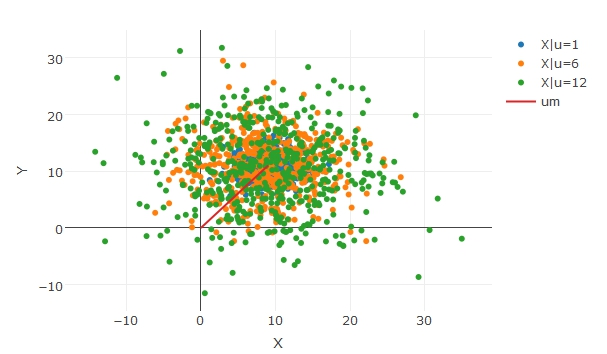
\includegraphics[width=1\linewidth]{Figuras/gvcarregida}
	\caption{Modelo de mezcla normal en varianza.}
	\label{fig:mez}
\end{figure}

\pagebreak
En la gráfica (\ref{fig:contornosv}) se observa cómo se modifican tanto la densidad como los contornos de la densidad de $X$ dado $u$ del ejemplo anterior. Claramente se observa que entre mayor sea el valor de $u$, mayor dispersión tendrá el vector $X$ dado $u$.



\begin{figure}[h]
	\centering
	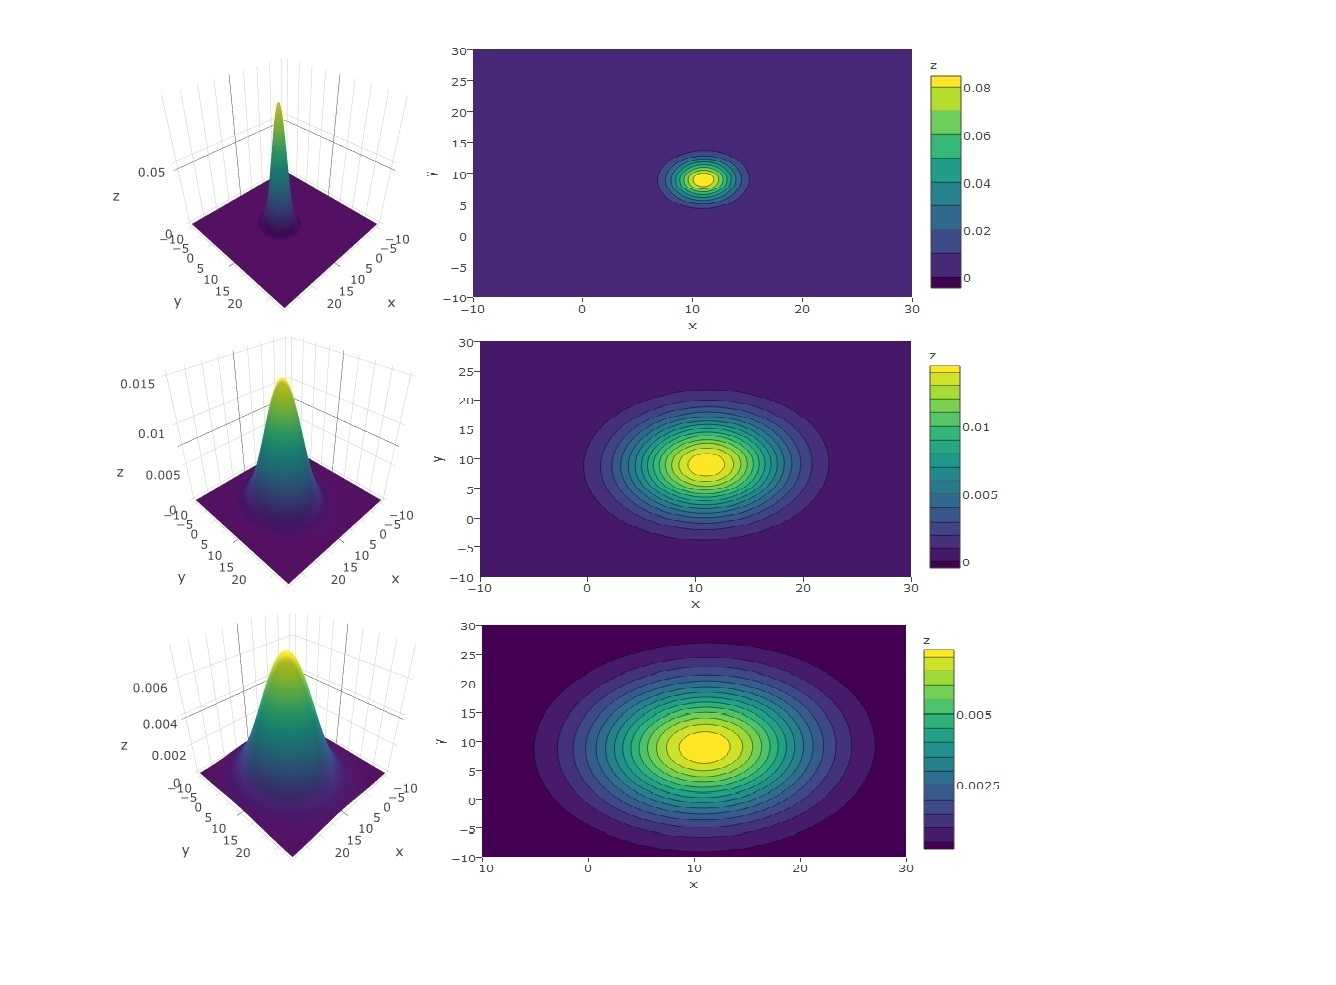
\includegraphics[width=1.15\linewidth]{Figuras/sv1}
	\caption{Contornos de una distribución tipo mezcla normal en varianza}
	\label{fig:contornosv}
\end{figure}
\pagebreak

Ahora considerando algunas características numéricas de $X$, y usando el anexo 4, es fácil probar que si $X$ se puede expresar como una distribución tipo mezcla normal en varianza, entonces: 

%\begin{equation*}
%E[X]=\mu
%\end{equation*}
%\begin{equation*}
%COV[X]=COV_{u}(E_{x}(X|u)) + E_{x}(COV_{u}(X|u))=E(u)\Sigma E(u)'
%\end{equation*}
\begin{eqnarray}
E[X]&=&\mu \nonumber \\
COV[X]&=&COV_{u}(E_{x}(X|u)) + E_{x}(COV_{u}(X|u)) \nonumber\\
&=&E(u)\Sigma E(u)'\nonumber\\
\end{eqnarray} 

Por lo que podemos conocer la esperanza y matriz de varianza-covarianza del vector $X$ con tan sólo conocer la matriz de varianza-covarianza de la distribución de $X$ dado $u$. Además, la distribución del vector $X$ estará centrada en el mismo vector de medias que $X$ dado $u$ para cualquier valor de $u$, mientras que la matriz de varianza-covarianza será proporcional a la matriz de varianza-covarianza de $X$ dado u.\\

En la gráfica (\ref{fig:dmv}) se presentan simulaciones de realizaciones del vector aleatorio $X$ a través de distribuciones tipo mezcla normal en varianza, para ello se utilizaron las mismas distribuciones de mezcla que en la gráfica (\ref{fig:abcd}). Adviértase que, a diferencia del condicionamiento en media, los datos solo se concentran alrededor del vector de medias $\mu$, pues $E[X]=E[X|u]$, perdiendo así la trayectoria que induce el vector de medias; intuitivamente podemos pensar que $u\mu$ del modelo de mezcla en media genera un vector de trayectoria para las observaciones de $X$, y que además induce un sesgo de las observaciones del vector $X$ sobre el vector de tendencia $\mu$.\\

\begin{figure}[h]
	\centering
	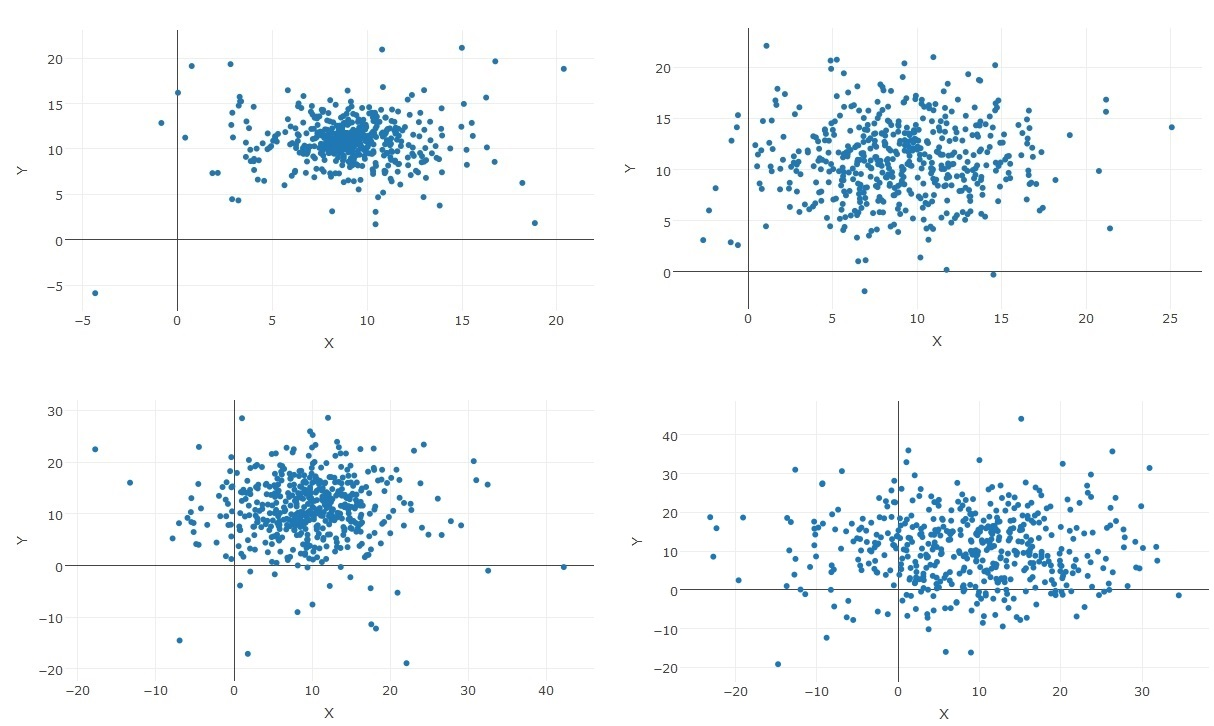
\includegraphics[width=1\linewidth]{Figuras/varianzaexp}
	\caption{Ejemplos de distribuciones tipo mezcla en varianza con diferentes distribuciones de mezcla.}
	\label{fig:dmv}
\end{figure}


\pagebreak
\section{Mezcla gaussiana en media-varianza}

Generalizando los dos modelos anteriores se tiene la siguiente definición:\\

Se dice que un vector aleatorio $X\in R^{p}$ es un vector tipo mezcla p-dimensional, si $X$ dado $u$ se ditribuye Normal con vector de medias $\mu +u\beta$, y matriz de varianza-covarianza $u\Sigma$, donde u es la variable de mezcla con soporte en $R_{+}$, $\mu, \beta \in R^{p}$ y $\Sigma\in M_{p \times p}$ matriz de varianza-covarianza.

Así pues, la distribución del vector $X$ está dada por:

\begin{equation*}
f_{X}(x)=\underset{S_{u}}{\int}\dfrac{1}{(2\pi)^{n/2}|u\Sigma|^{n/2}}\exp(-\dfrac{1}{2}(x-\mu-uB)\acute{}u\Sigma^{-1}(x-\mu-uB))f(u)du 
\end{equation*}

Si nos concentramos en la distribución marginal de $X$ dado $u$, notamos que ahora, para cada realización  $u_{i}$, la densidad de $X$ dado $u_{i}$ estará centrada en el vector $\mu + u_{i}\beta$, y conforme $u_{i}$ tome valores más grandes, la densidad de $X/u_{i}$ se desplazará en dirección del vector $u_{i}\beta$ cada vez con mayor dispersión. 
En la gráfica (\ref{fig:dmnev}) se puede observar una variable tipo mezcla en esperanza varianza, con parámetros $\beta=(9,11)$, $\mu=(5,10)$, y matriz de varianza-covarianza $\Sigma$
con $\sigma_{z}=\sigma_{y}=5$, y $COV(Z,Y)=0$.$1$, donde $X=(Z,Y)$ es un vector aleatorio de dimensión $2$.
%$\left(
%\begin{array}{lcr}
%5 & .1 \\ . 1 & 5
%\end{array}\right) 
. La variable de mezcla $u$ se distribuye exponencial y tomó los valores de $1$, $3$ y $6$ respectivamente.

\begin{figure}[h]
	\centering
	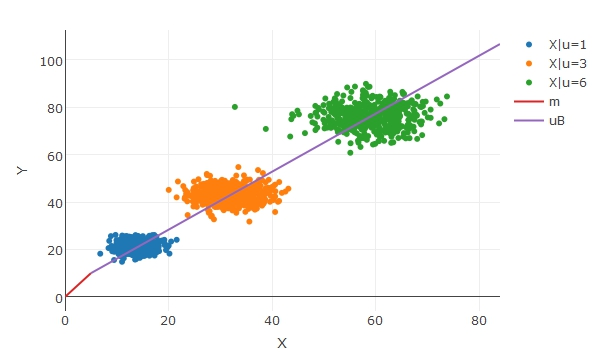
\includegraphics[width=1\linewidth]{Figuras/bm}
	\caption{Gráfica de una variable tipo mezcla normal en esperanza varianza}
	\label{fig:dmnev}
\end{figure}


\pagebreak
En la distribución de $X$ podemos considerar a $\mu$ como un vector de posición, mientras que $u\beta$ es un vector de dirección o tendencia alrededor del cual estarán las observaciones de $X$. Los datos conservarán la estructura de correlación inherenta a $\Sigma$, pero además estarán dispersos en proporción a la esperanza de la variable de mezcla $u$, más alguna constante que depende de $u$. Siguiendo la idea intuitiva del modelo de mezcla en media, el producto de la variable de mezcla $u$ y el vector $\beta$ inducen un sesgo en cada realización del vector aleatorio $X$. Entonces, considerando el anexo 4,  la esperanza y covarianza del vector $X$ tienen la forma:

\begin{eqnarray}
E(X)&=&E_{u}(E_{x}(x|u)) \nonumber\\
&=&E_{u}(\mu + u\beta)\nonumber\\
&=&\mu+E(u)\beta\nonumber\\
COV(X)&=&COV_{u}(E_{x}(X|u)) + E_{u}(COV_{x}(X|u)) \nonumber\\
&=&COV_{u}(\mu + u\beta) + E_{u}(u\Sigma) \nonumber\\
&=&Var(u)\beta \beta' + E(u)\Sigma \nonumber\\
\end{eqnarray}
%\begin{equation*}
%E(X)=E_{u}(E_{x}(x|u))=E_{u}(\mu + u\beta)=\mu+E(u)\beta
%\end{equation*}
%\begin{equation*}
%COV(X)=COV_{u}(E_{x}(X|u)) + E_{u}(COV_{x}(X|u))=
%\end{equation*}
%\begin{equation*}
%COV_{u}(\mu + u\beta) + E_{u}(u\Sigma)=Var(u)\beta \beta' + E(u)\Sigma
%\end{equation*}

Y además, como se verá posteriormente, la función generadora de momentos $M_{x}(t)$ del vector aleatorio X es proporcional a $M_{u}(t)$, la función generadora de momentos de la variable de mezcla u. Y la función característica $\Phi_{x}(it)$ es proporcinal a la función característica de la variable de mezcla u, $\Phi_{u}(it)$.\\


\section{Propiedades en mezclas de media-varianza}

1) La función característica de $X$ es: 
\begin{equation*}
\Phi_{X}(t)=\exp \left( it\mu\acute{} \right) \Phi_{u}(it\beta\acute{}-\frac{1}{2}t\Delta t\acute{}) 
\end{equation*}
Donde $\Phi_{u}(.)$ es la función característica de la variable de mezcla $u$. \\

Demostración:\\

\begin{eqnarray}
\Phi_{X}(t)&=&\underset{x}{\int }\exp(it)f(x)dx \nonumber\\
&=& \underset{x}{\int }\exp(it)(\underset{u}{\int}f(x|u)f(u)du)dx\nonumber\\
&=&\underset{x}{\int}\underset{u}{\int}exp(it)f(x|u)f(u)dudx\nonumber\\
\end{eqnarray}
%\begin{equation*}
%\Phi_{X}(t)=\underset{x}{\int }\exp(it)f(x)dx = \underset{x}{\int }\exp(it)(\underset{u}{\int}f(x|u)f(u)du)dx=
%\end{equation*}
%\begin{equation*}
%\underset{x}{\int}\underset{u}{\int}exp(it)f(x|u)f(u)dudx
%\end{equation*}

\begin{eqnarray}
\underset{x}{\int}\underset{u}{\int}exp(it)f(x)|_{u}f(u)dudx&=&\underset{u}{\int}\underset{x}{\int}exp(it)f(x)|_{u}f(u)dudx \nonumber \\
\end{eqnarray}
\begin{equation*}
=\underset{u}{\int}exp(it(\mu+ u\beta)+\frac{1}{2}itu\Delta it)f(u)du
\end{equation*}
%\begin{equation*}
%\underset{x}{\int}\underset{u}{\int}exp(it)f(x)|_{u}f(u)dudx=\underset{u}{\int}\underset{x}{\int}exp(it)f(x)|_{u}f(u)dudx=
%\end{equation*}
%\begin{equation*}
%\underset{u}{\int}exp(it(\mu+ u\beta)+\frac{1}{2}itu\Delta it)f(u)du
%\end{equation*}


Ya que la función generadora de momentos de una distribución Normal p-variada es $exp(t\acute{}\mu + t\acute{}\Sigma t)$, y además $X$ dado $u$ se distribuye $N(\mu + u\beta, u\Delta)$ \\

Factorizando el exponenete de la exponencial se tiene que:\\
\begin{eqnarray}
\underset{u}{\int}exp(it(\mu+ u\beta)&+&\frac{1}{2}itu\Delta it)f(u)du=\nonumber\\
&=&\underset{u}{\int}\exp(it\acute{}\mu)exp(u(it\acute{}\beta -\dfrac{1}{2}t\acute{}u \Delta t))f(u)du\nonumber\\
&=&exp(it\acute{}\mu)\Phi_{u}(it\beta-\frac{1}{2}t\Delta t)\nonumber\\
\end{eqnarray}

%\begin{equation*}
%\underset{u}{\int}exp(it(\mu+ u\beta)+\frac{1}{2}itu\Delta it)f(u)du=
%\end{equation*}
%\begin{equation*}
%\underset{u}{\int}\exp(it\acute{}\mu)exp(u(it\acute{}\beta -\dfrac{1}{2}t\acute{}u \Delta t))f(u)du = exp(it\acute{}\mu)\Phi_{u}(it\beta-\frac{1}{2}t\Delta t)
%\end{equation*}
Por lo tanto: 
\begin{equation*}
\Phi_{X}(t) = exp(it\acute{}\mu)\Phi_{u}(it\beta-\frac{1}{2}t\Delta t)
\end{equation*}

Para comprobar que la función generadora de $X$ es:
\begin{equation*}
M_{x}(t)=\exp^{t\acute{}\mu}M_{u}(t\beta+\dfrac{1}{2}t\acute{}\Delta t)
\end{equation*}
basta con sustituir $t$ por $it$ en el resultado anterior.\\

El resultado anterior nos indica que podemos obtener la función generadora de momentos o característica del vector aleatorio $X$ con tan solo conocer la función característica o generadora de la variable de mezcla $u$, lo cual sería de utilidad si sólo nos interesan algunos momentos, o también nos ayudaría a identificar la distribución de $X$, en caso de reconocer la función característica o generadora de momentos. Inversamente, el resutado anterior indica que si la función característica o generadora de algún vector aleatorio $Z$ se puede descomponer como el producto de $\exp{it\acute{}\mu} $, y alguna $M_{y}(t)$, entonces $Z$ es una variable normal de mezcla en esperanza-varianza, con distribución de mezcla $y$.\\

\section{Distribución hiperbólica generalizada}
La familia paramétrica Hiperbólica Generalizada se obtiene a partir de definir una mezcla Noramal en esperanza varianza, donde el vector aleatorio $X$ de dimensión $p$ condicionado en $u$ tiene una distribución Normal con vector de esperanza $\mu +u\beta$, y matriz de varianza covarianza $u\Sigma$, mientras que la variable de mezcla $u$ se distribuye Gaussiana inversa generalizada con parámetros $\Psi$ y $\lambda$, por lo que formalmente la función de densidad del vector aleatorio $X$ queda de la siguiente forma:\\


Se dice que el vector aleatorio $X$ $p$-variado tiene una distribución Hiperbólica Generalizada  si su densidad es de la siguiente manera:

\begin{eqnarray*}
f_{X}(x|\lambda,\xi,\Psi,\mu,\Sigma,\beta)&=&c\frac{\kappa_{\lambda-d/2}(\sqrt{\xi +(x-\mu)'\Sigma^{-1}(x-\mu)(\Psi+\beta\acute{}\Sigma^{-1}\beta)})}{\xi + (x-\mu)'\Sigma^{-1}(x-\mu)(\Psi+\beta'\Sigma^{-1}\beta)^{\frac{d}{2}-\lambda}}\\
& &\exp{(x-\mu)'\Sigma^{-1}\beta},\\
\end{eqnarray*}
donde $c=\frac{\sqrt{\xi\lambda}^{-\lambda}\Psi^{\lambda}(\Psi+\beta\acute{} \Sigma^{-1}\beta)^{\frac{d}{2}-\lambda}}{(2\Pi)^{\frac{d}{2}}|\Sigma|^{\frac{1}{2}}\kappa_{\lambda(\sqrt{\xi\Psi})}}$. \\

Si el vector aleatprio $X$ tiene una distribución Hiperbólica Generalizada usaremos la notación
$X$ se distribuye $GH_{p}(\lambda,\xi,\Psi,\mu,\Sigma,\beta)$.\\

La distribución Hiperbólica generalizada se caracteriza a partir de una mezcla normal en esperanza y varianza de la siguiente manera: se $X$ dado $u$ un vector aleatorio de dimensión $p$ que se distribuye $N(\mu+u\beta,u\Sigma)$, y sea $u$ la variable de mezcla distribuida $N\bar{}(\lambda,\xi,\Psi)$, entonces:
%\begin{eqnarray*}
%f_{x}(X) & = &\underset{-\infty }{\overset{\infty }{\int }}\frac{\exp{(x-\mu)'\Sigma^{-1}(x-\mu)}}{(2\Pi)^{d/2}|\Sigma|^{1/2}u^{d/2}}\end{eqnarray*}\\
%& &\exp{-
%\dfrac{(x-\mu)'\Sigma^{-1}(x-\mu)}{2u}}-\frac{\beta\Sigma^{-1}\beta}{2/u}f(u)du,\\
%\end{eqnarray*}
\begin{eqnarray*}
f_{X}(x|\lambda,\xi,\Psi) & = &\underset{-\infty }{\overset{\infty }{\int }}\frac{\exp{(x-\mu)'\Sigma^{-1}(x-\mu)}}{(2\Pi)^{d/2}|\Sigma|^{1/2}u^{d/2}}\\
& & \exp{-
	\dfrac{(x-\mu)'\Sigma^{-1}(x-\mu)}{2u}}-\frac{\beta\Sigma^{-1}\beta}{2/u}f(u)du,\\
\end{eqnarray*}
donde:
\begin{equation*}
f(u)=\dfrac{\xi^{-\lambda}\sqrt{\xi\Psi}^{\lambda}u^{\lambda-1}\exp{\frac{-1}{2}(\xi u^{-1} + \Psi u)}}{2\kappa_{\lambda}(\sqrt{\xi\Psi})} 
\end{equation*}

Sea $a=(x-\mu)'\Sigma^{-1}(x-\mu)$, y $b=\beta\Sigma^{-1}\beta$, entonces de aquí se sigue que:

\begin{eqnarray*}
f(x)&=&\frac{\exp{(x-\mu)'\Sigma^{-1}\beta}\xi^{-\lambda}\sqrt{\xi\Psi}^{\lambda}}{(2\Pi)^{d/2}|\Sigma|^{1/2}2k_{\lambda}(\sqrt{\xi\Psi})}\\
& & \underset{-\infty }{\overset{\infty }{\int }}u^{\lambda - d/2 -1}\exp{-1/2(au^{-1}bu+\xi u^{-1}+\Psi u)}du\\
\end{eqnarray*}

Trabajando solamente con el integrando se tiene que:

\begin{eqnarray*}
& &\underset{-\infty }{\overset{\infty }{\int }}u^{\lambda - d/2 -1}\exp{-1/2(au^{-1}+bu+\xi u^{-1}+\Psi u)}du\\
&=&\underset{-\infty }{\overset{\infty }{\int }}u^{\lambda -d/2 -1}\exp{-1/2((a+\xi)u^{-1}+(b+\Psi)u} du\\
\end{eqnarray*}



Ahora, sea $\lambda\acute{}=\lambda- 1/2$, $\xi\acute{}=a+\xi$, $\Psi\acute{}=b+\Psi$, entonces:

\begin{eqnarray*}
& &\underset{-\infty }{\overset{\infty }{\int }}u^{\lambda -d/2 -1}\exp{-1/2((a+\xi)u^{-1}+(b+\Psi)u} du\\
&=&\underset{-\infty }{\overset{\infty }{\int }}u^{\lambda'-1}\exp{-1/2(\xi' u^{-1}+ \Psi'u)} du
\end{eqnarray*}
luego,

\begin{equation*}
\underset{-\infty }{\overset{\infty }{\int }}u^{\lambda'-1}\exp{-1/2(\xi' u^{-1}+ \Psi'u)} du=     \frac{2k_{\lambda'}(\sqrt{\xi'\Psi'})}{\xi'^{-\lambda'}(\sqrt{\xi'\Psi'})^{\lambda'}}   \underset{-\infty }{\overset{\infty }{\int }}\frac{\xi^{-\lambda'}(\sqrt{\xi\Psi})^{\lambda'}}{2k_{\lambda'}(\sqrt{\xi'\Psi'})}
\end{equation*}
\begin{equation*}
u^{\lambda'-1}\exp{-1/2(\xi' u^{-1}+ \Psi'u)} du
\end{equation*}

Donde la última integral vale uno por ser una distribución $N\bar{}(\lambda\acute{},\xi\acute{},\Psi\acute{})$ integrada sobre su soporte, por lo que tenemos que:\\

\begin{equation*}
f(x)=\frac{\exp{(x-\mu)'\Sigma^{-1}\beta}\xi^{-\lambda}\sqrt{\xi\Psi}^{\lambda}}{(2\Pi)^{d/2}|\Sigma|^{1/2}2k_{\lambda}(\sqrt{\xi\Psi})}\frac{2k_{\lambda'}(\sqrt{\xi'\Psi'})}{\xi^{-\lambda'}(\sqrt{\xi'\Psi'})^{\lambda'}}
\end{equation*}\\

Por último, sustituyendo los valores de $a$, $b$, $\xi\acute{}$, $\Psi\acute{}$, y agrupando algunos términos tenemos que efectivamente $X$ se distribuye $GH_{p}(\lambda,\xi,\Psi,\mu,\Sigma,\beta)$.\\

Ahora para encontrar los momentos de la distribución $GH_{p}$, como puede ser expresada como una variable de mezcla en esparanza-varianza, la propiedad 1) nos dice que $\Phi_{X}(t)=\exp(it\beta\mu\acute{})\Phi_{u}(it\beta\acute{}-\frac{1}{2}t\Sigma t\acute{})$, donde $\Phi_{u}(.)$ es la función característica del la variable de mezcla u que se distribuye $N\bar{}(\lambda,\xi,\Psi)$.\\

La función característica nos permite calcular fácilmente la distribución de una transformación lineal del vector p-variado $X$, pues si ahora consideramos el vector aleatorio $Y=aX+b$, donde $a\in M_{rxp}$, $b\in R^{p}$ entonces:

\begin{eqnarray*}
\Phi_{Y}(t) &=&exp(bit)\Phi_{X}(at)\\
&=&\exp(bit+it\beta\mu\acute{})\Phi_{u}(iat\beta\acute{}-\frac{1}{2}at\Sigma at\acute{})\\
&=& \exp(it(b+\beta\mu)\acute{})\Phi_{u}(iat\beta\acute{}-\frac{1}{2}at\Sigma at\acute{})\\
\end{eqnarray*}

Lo cual nos indica que $Y$ se distribuye $GH_{p}(\lambda,\xi,\Psi,b+\beta\mu,a\Sigma a\acute{},a\beta)$, y a su vez que.\\

También a partir de la función característica es fácil ver que la distribución marginal de $X_{i}$ es 
$GH_{p}(\lambda,\xi,\Psi,\mu_{i},\Sigma _{i},\beta_{i})$, donde $\Sigma_{i}$ es el i-ésimo componente del primer renglón de $\Sigma$. Las dos propiedades anteriores nos dicen que si X se distribuye $GH_{p}$, entonces es cerrado bajo convoluciones.

